\documentclass{beamer}
% \usepackage[brazil]{babel}
\usepackage[utf8]{inputenc}
\usepackage{fancybox}
\title[Teaching]{Teaching}
%\subtitle[short version]{}
%\date{}
\author[Sivaram Ambikasaran]{Sivaram Ambikasaran}
\institute[IITM]{Indian Institute of Technology Madras}
\usetheme{Madrid}


 
\usecolortheme{owl}
\setbeamercolor{normal text}{fg=orange}
\usebeamercolor*{normal text}
\setbeamerfont{frametitle}{size=\Huge}

\begin{document}
\frame{\titlepage}


\begin{frame}{Teaching Philosophy}
	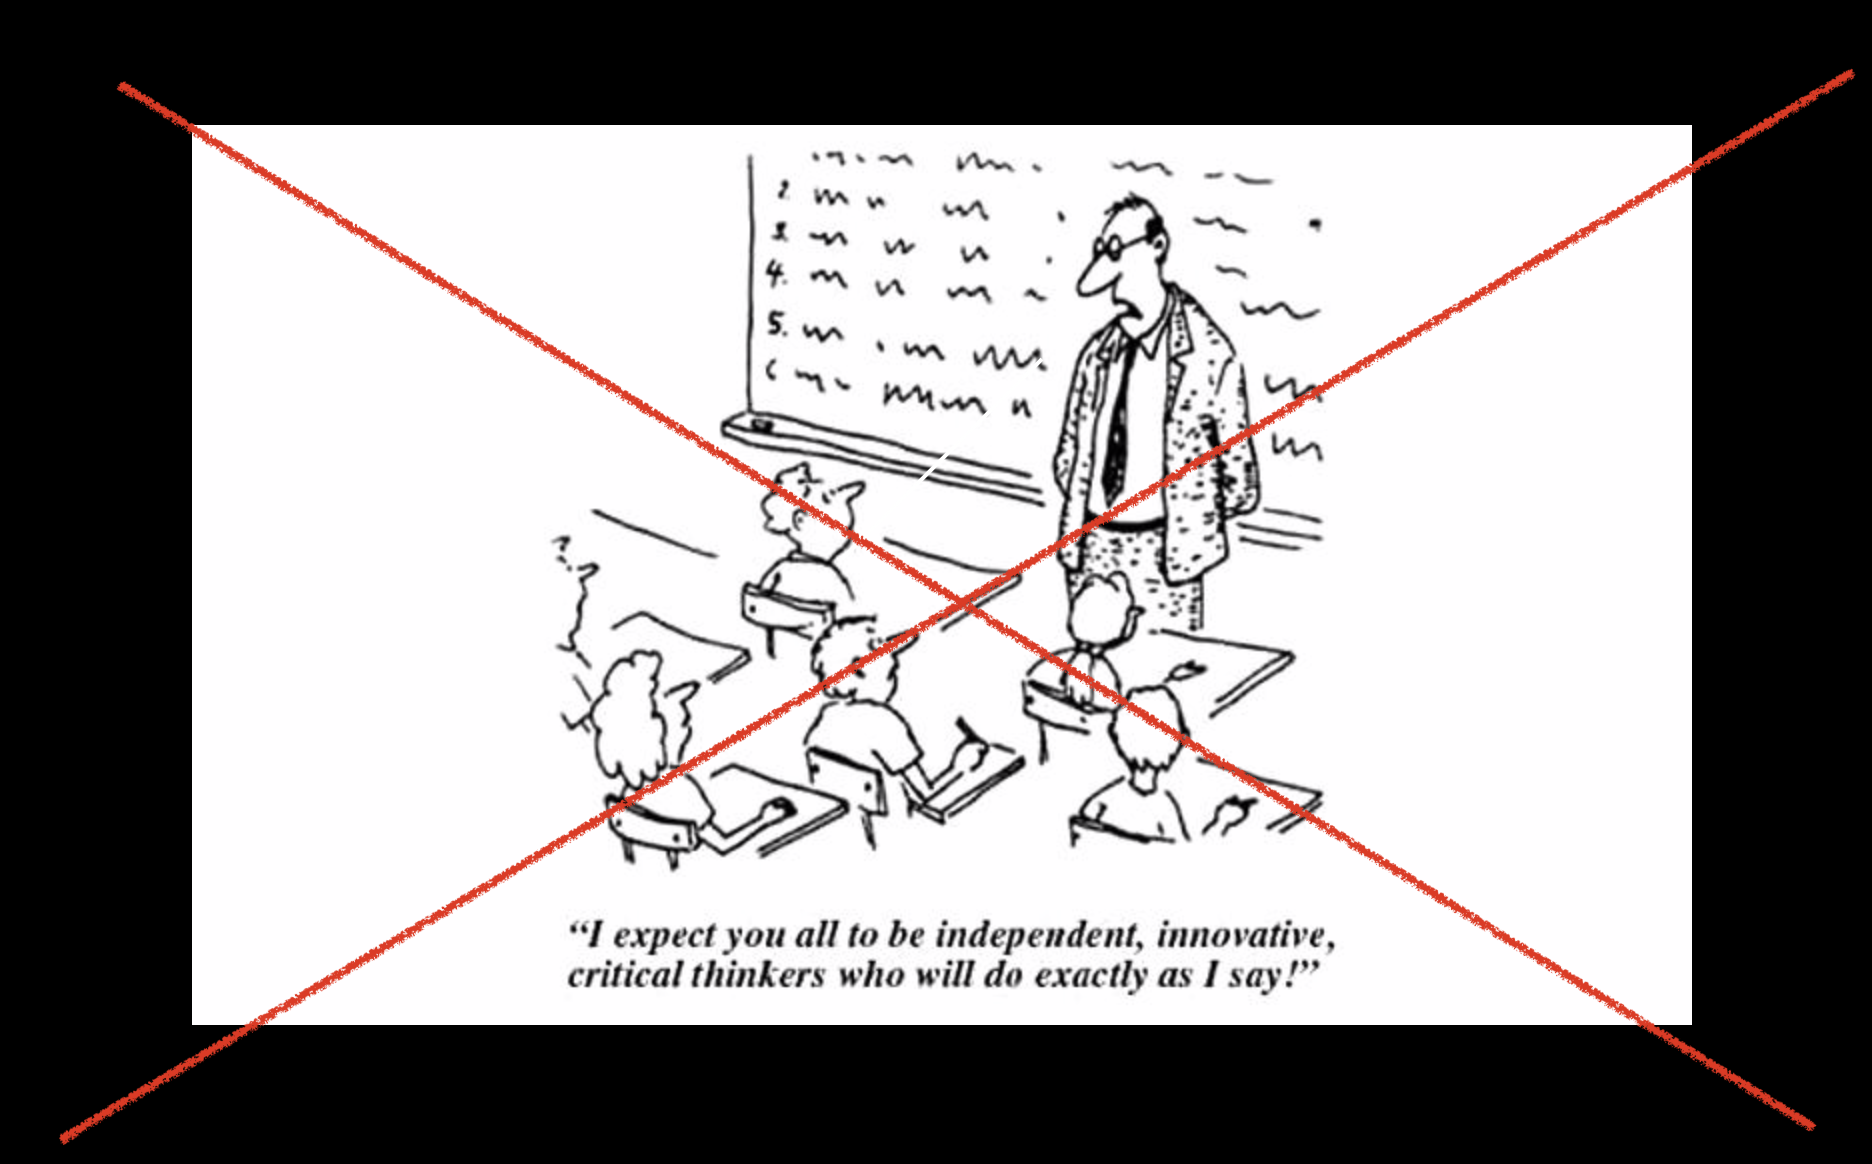
\includegraphics[width=\textwidth]{./images/Comic_Teaching.png}
\end{frame}

\begin{frame}[c]{Teaching Philosophy}
	\begin{center}
	\Huge{Teacher, Professor?}\\
	\pause
	\vspace{2em}
	\Huge{I am an {\color{cyan}educational} {\color{magenta}rockstar}}
	\end{center}
\end{frame}

\begin{frame}[c]{Teaching Philosophy}
	\LARGE
	\begin{center}
		``Intellectually entertain students and make them learn"\\
	\vspace{1em}
	``Don’t try to teach, try to make the students learn”\\
	\vspace{1em}
	``Try to figure things out along with the students"
	\end{center}
\end{frame}

\begin{frame}[c]{Teaching Philosophy}
	\LARGE
	\begin{itemize}
		\item
		Spend the first lecture on motivation
		\item
		Why, What and How?
		\item
		Numerical Linear Algebra
		\begin{itemize}
			\item
			The \$25,000,000,000 Eigenvector: Linear algebra behind google
			\item
			The Smart Money’s on Numerical Analysts
		\end{itemize}
	\end{itemize}
\end{frame}

\begin{frame}[c]{Teaching Philosophy}
	\LARGE
	Adopt latest technologies in teaching
	\begin{center}
	
\includegraphics[width=0.2\textwidth]{./images/Github.png} \hspace{1em}
	
\includegraphics[width=0.45\textwidth]{./images/Jupyter.png}\\
	\vspace{1em}
	
\includegraphics[width=0.45\textwidth]{./images/AutoGradr.png} \hspace{1em}
	
\includegraphics[width=0.45\textwidth]{./images/JPlag.png}
	\end{center}
\end{frame}

\begin{frame}{Finite Precision Computation}
	\LARGE
	Solving recurrence
	$$a_{n+1} = 10a_n - 9a_{n-1}$$
	with $a_0 = a_1 = 2.95$
\end{frame}

\begin{frame}{Polynomial Approximation}
	\LARGE
	Interpolate/Approximate
	$$f(x) = \dfrac1{1+25x^2}$$
	Weierstrass approximation theorem
\end{frame}

\begin{frame}{MonteCarlo to compute $\pi$}
	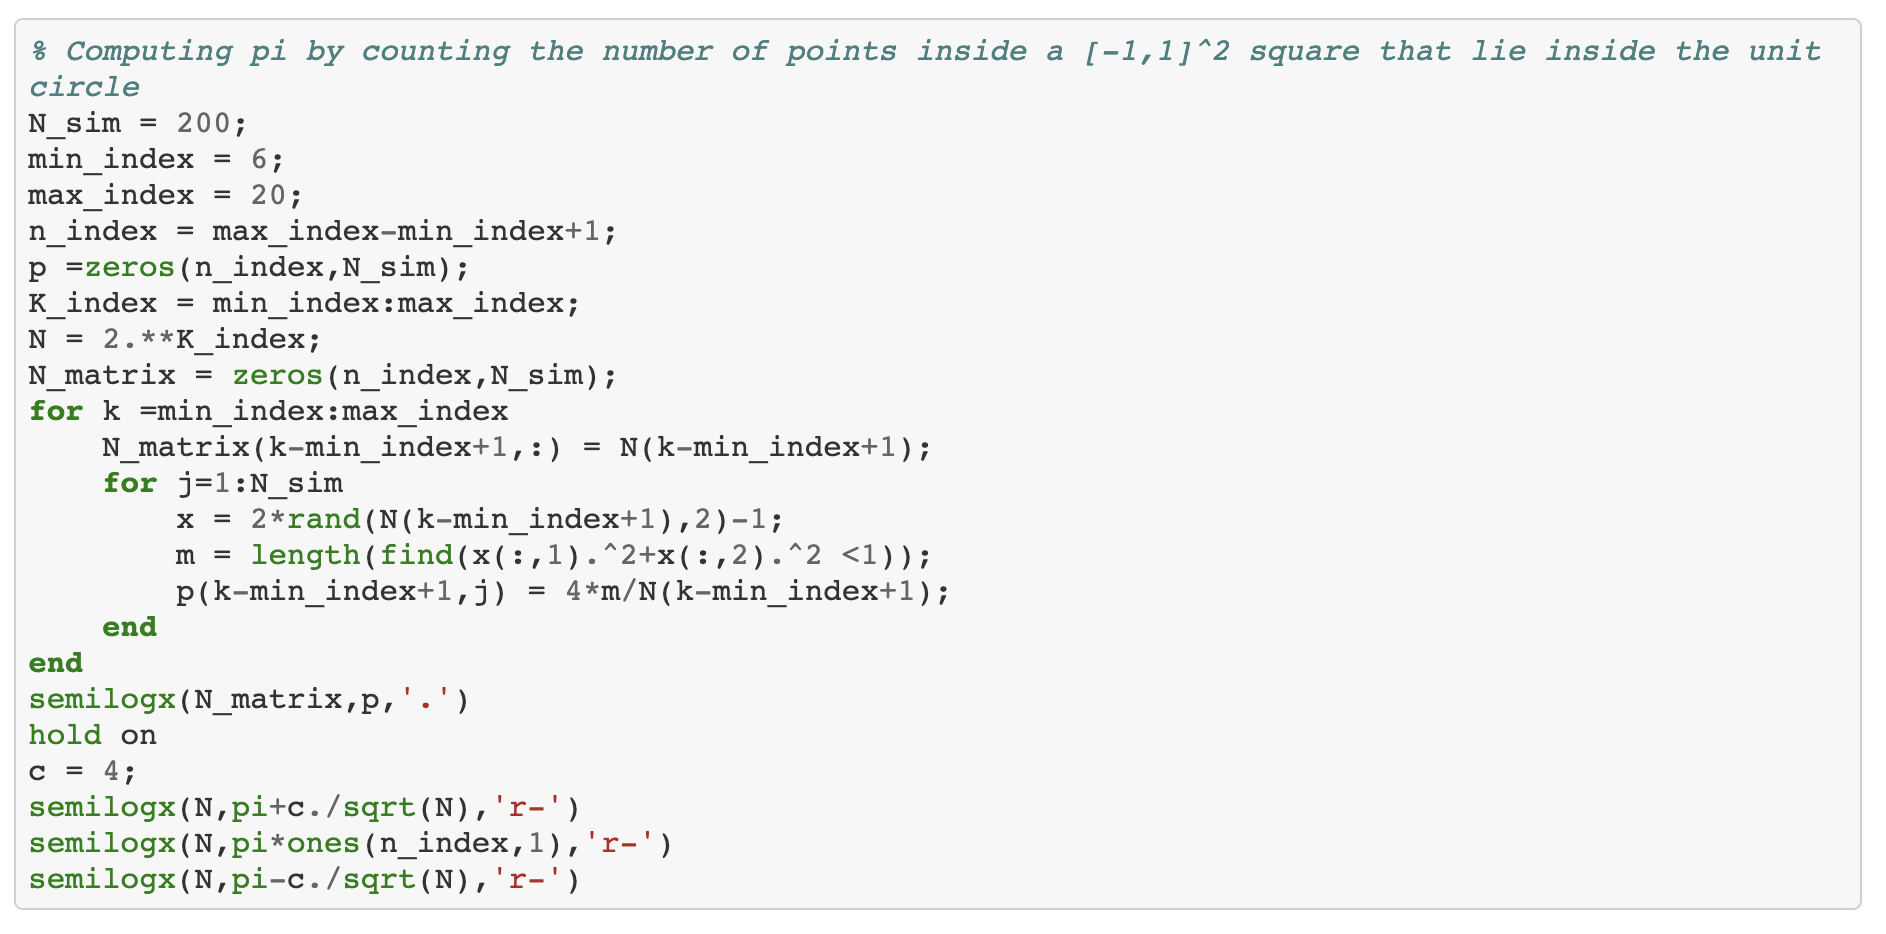
\includegraphics[width=\textwidth]{./images/pi_1.png}
\end{frame}

\begin{frame}{MonteCarlo to compute $\pi$}
	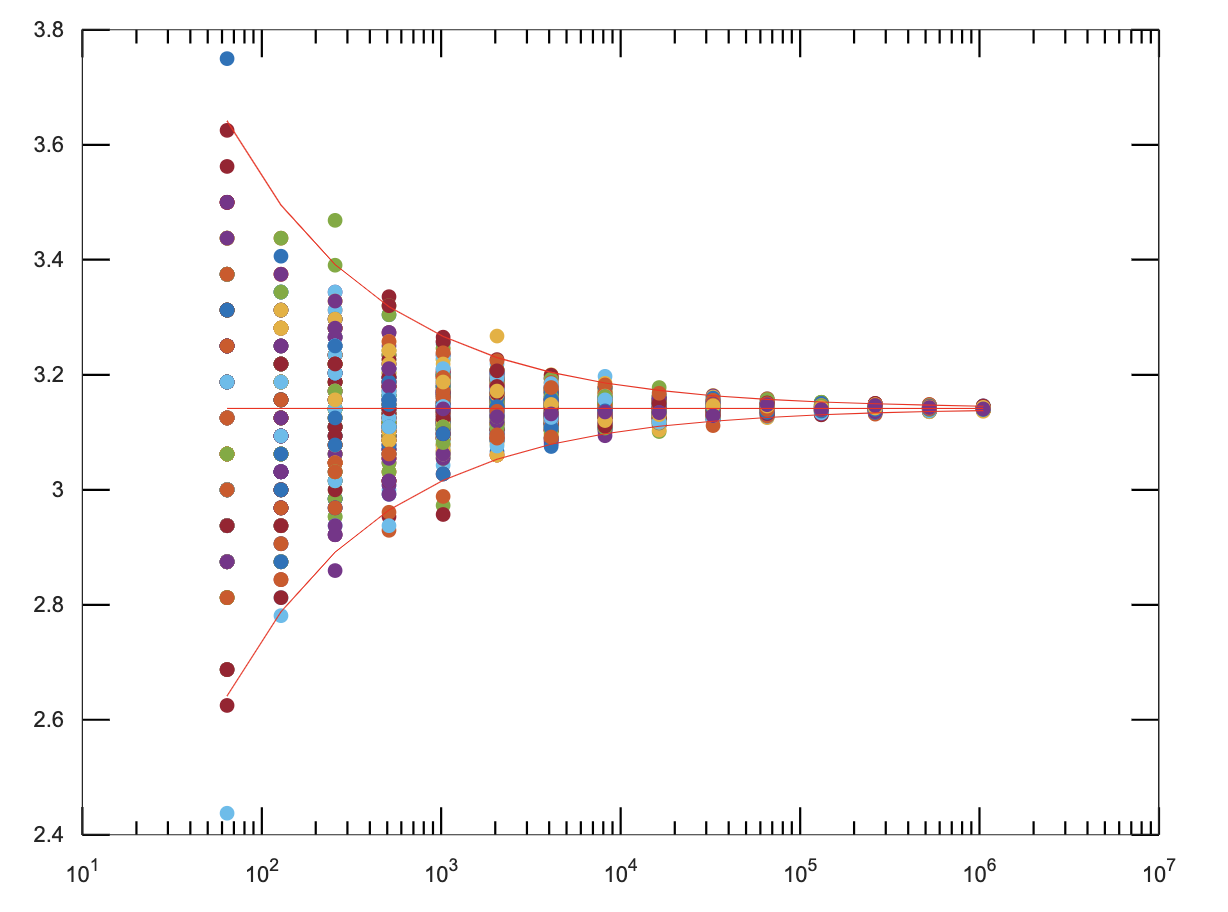
\includegraphics[width=\textwidth]{./images/pi_2.png}
\end{frame}

\begin{frame}{Summary of teaching philosophy}
	\large
	To heighten the understanding of concepts
	\begin{itemize}
		\item
		Proofs and more importantly examples/counterexamples
		\item
		Application of the theorems/results
		\item
		Live computational and mathematical demonstrations
		\begin{itemize}
			\item
			Students appreciate that math and programming can go hand in hand
			\item
			Both are simple and fun to play around
		\end{itemize}
		\pause
		\item
		Will think along with students for the logic to be followed
		\item
		Enable them to think on the fly and adapt; contributes to their understanding
	\end{itemize}
	These enable students to understand the details as well as to obtain a bird's eye view of the entire landscape.
\end{frame}
\end{document}